\section{Theoretical Analysis}
\label{sec:analysis}
In this section, the circuit shown in Figure~\ref{fig:circuit} is analysed
theoretically. We will begin by analyzing the Gain Stage circuit and, after that, the Output Stage circuit.
%in order to predict their outputs. 
Thus, we will start by computing the Operating Point using the theoretical DC
model studied and comparing it to Ngspice’s OP.

Then, we will compute the gain and input and output impedances separately for the 2 stages. 

Finally, we will compute the frequency response Vo(f)/Vi(f).

%The theoretical values will be obtained by applying Kirchhoff laws and the diode equations.
%Considering the circuit of Figure~\ref{fig:circuit}, it is composed by a Voltage source, a transformer, an envelope detector and a voltage regulator.
%--------------------------------------------------------------------------------------------
\subsection{Gain Stage}
In this subsection, we will analyze the Gain Stage circuit. Its function is to ensure a high input voltage so that the input signal is not degraded or distorted throughout the circuit. It also has a high gain associated, being responsible for amplifying the signal.

In order to make the analysis task easier, we used Thévenin's equivalent of bias circuit. Its diagram is represented in Figure~\ref{fig:gscircuit} as well as the NPN BC547A model used in this assignment is shown in table~\ref{tab:bgs}.

\begin{figure}[H] \centering
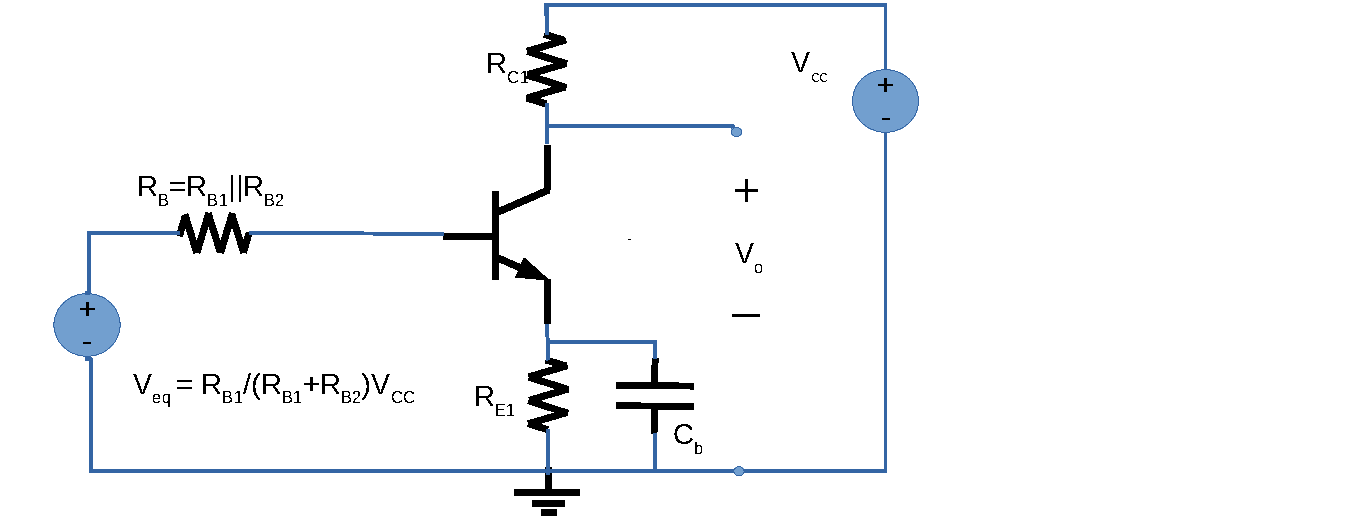
\includegraphics[width=0.8\linewidth]{gainstage.pdf}
\caption{Gain Stage Circuit}                                     %%%%%%%%%%LEGENDA
\label{fig:gscircuit}
\end{figure}

\begin{table}[H]
  \centering
  \begin{tabular}{|l|r|}
     \hline    
    {\bf Name} & {\bf Value} \\ \hline   
    $V_{T}$ & 0.025000 V\\ \hline
$beta$ & 178.700000 \\ \hline
$V_{A}$ & 69.700000 V\\ \hline
$V_{BEON}$ & 0.700000 V \\ \hline

  \end{tabular}
  \caption{BC547A model}
  \label{tab:bgs}
\end{table}

In gain stage circuit, it is important to mention that capacitor $C_I$ is a coupling capacitor, acting as a DC Block, and $C_b$ is a bypass capacitor.

\subsubsection{Operating Point}
Considering the equations of the lecture 17 and the theoretical DC model studied , we compute the OP. The table~\ref{tab:opgs} presents the results obtained.

\begin{table}[H]
  \centering
  \begin{tabular}{|l|r|}
     \hline    
    {\bf Name} & {\bf Value} \\ \hline   
    $R_{B}$ & 1.600000e+04 Ohm\\ \hline
$V_{eq}$ & 2.400000e+00 V\\ \hline
$I_{B1}$ & 1.094885e-05 A \\ \hline
$I_{C1}$ & 1.956559e-03 A \\ \hline
$I_{E1}$ & 1.967508e-03 A \\ \hline
$V_{E1}$ & 1.524818e+00 V \\ \hline
$V_{O1}$ & 1.016083e+01 V \\ \hline
$V_{CE}$ & 8.636016e+00 V \\ \hline

  \end{tabular}
  \caption{OP - Gain Stage}
  \label{tab:opgs}
\end{table}

\subsubsection{Gain and Input and Output Impedances}
Then, we will compute the gain and input and output impedances. In order to do that, we will  use the incremental circuit, whose diagram is represented in Figure~\ref{fig:gsincrem}.

\begin{figure}[H] \centering
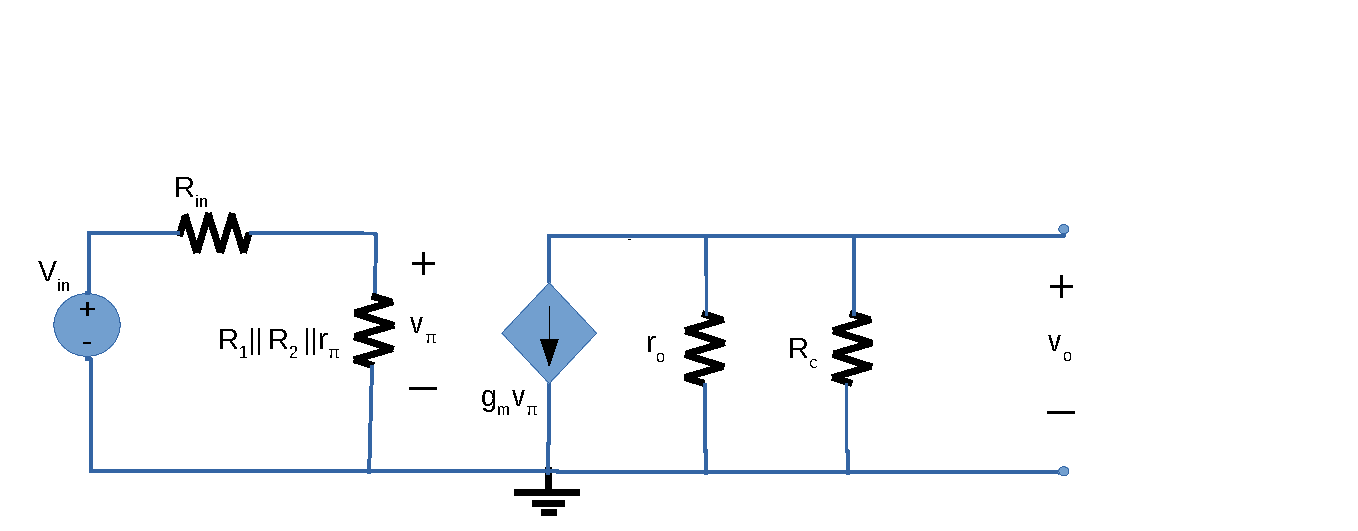
\includegraphics[width=0.8\linewidth]{incrementalgs.pdf}
\caption{Incremental Gain Stage Circuit}                         %%%%%%%%%%LEGENDA
\label{fig:gsincrem}
\end{figure}

Starting by calculating the gain, after analyzing the circuit, we obtain the following equation: 
\begin{equation}
	A_v=\frac{v_o}{v_{in}}=-g_m(r_o||R_C)\frac{R_B||r_\pi}{R_B||r_\pi+R_{in}}
\end{equation}

Notice that the capacitor $C_b$ was used to bypass $R_E$. Otherwise, the gain will be lower and the lower cutoff frequency too high. This way, CE is an open-circuit for low frequency (DC) and a short-circuit fot higher frequencies (AC).

Table~\ref{tab:avgs} presents the results.

\begin{table}[H]
  \centering
  \begin{tabular}{|l|r|}
     \hline    
    {\bf Name} & {\bf Value} \\ \hline   
    $A_{V1}$ & 3.668323e+01 dB\\ \hline

  \end{tabular}
  \caption{Gain - Gain Stage}
  \label{tab:avgs}
\end{table}

In order to obtain the impedances, we used the following equations:
\begin{equation}
	Z_{I1}=R_B1||R_B2||r_\pi
\end{equation}
\begin{equation}
	Z_{O1}=R_C||R_o
\end{equation}

The results are presented in Table~\ref{tab:zgs}
\begin{table}[H]
  \centering
  \begin{tabular}{|l|r|}
     \hline    
    {\bf Name} & {\bf Value} \\ \hline   
    $Z_{I1}$ & 1.998186e+03 Ohm\\ \hline
$Z_{O1}$ & 9.158340e+02 Ohm\\ \hline

  \end{tabular}
  \caption{Input and Output Impedances - Gain Stage}
  \label{tab:zgs}
\end{table}

Notice that, in this section, we have made the approximation $R_E1 \approx 0$, because it is assumed the capacitors are shor-circuited, i.e. high frequency analysis.

Finally, we should pay attention to the values of the output impedance of gain stage. Its values are high when compared with the load. That's why we need the Output Stage.
%--------------------------------------------------------------------------------------------
\subsection{Output Stage}
In this subsection, we will analyze the Output Stage circuit, wich presents a lower output impedance. Its diagram is represented in Figure~\ref{fig:oscircuit} as well as the PNP BC547A model used in this assignment is shown in table~\ref{tab:modelos}.

\begin{figure}[H] \centering
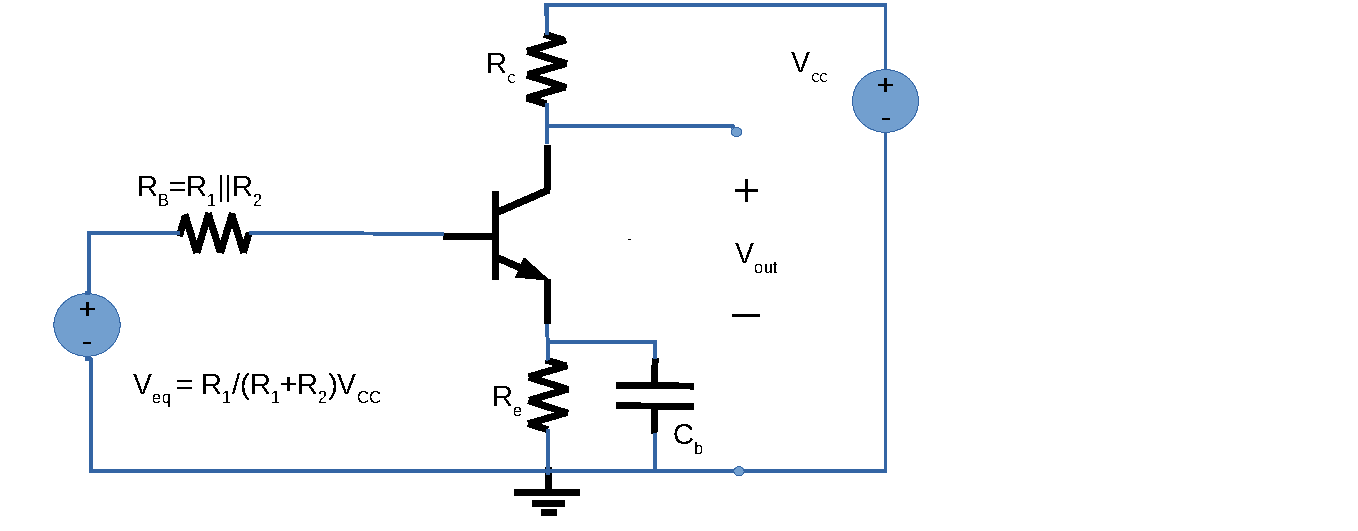
\includegraphics[width=0.8\linewidth]{outstage.pdf}
\caption{Output Stage Circuit}                                     %%%%%%%%%%LEGENDA
\label{fig:oscircuit}
\end{figure}

\begin{table}[H]
  \centering
  \begin{tabular}{|l|r|}
     \hline    
    {\bf Name} & {\bf Value} \\ \hline   
    $beta$ & 227.300000 \\ \hline
$V_{AFP}$ & 37.200000 V\\ \hline
$V_{BEON}$ & 0.700000 V \\ \hline

  \end{tabular}
  \caption{BC557A model}
  \label{tab:modelos}
\end{table}

\subsubsection{Operating Point}
Considering the equations of the lecture 17, we compute the OP. The table~\ref{tab:osop} presents the results obtained.

\begin{table}[H]
  \centering
  \begin{tabular}{|l|r|}
     \hline    
    {\bf Name} & {\bf Value} \\ \hline   
    $V_{I2}$ & 1.016083e+01 V\\ \hline
$I_{E2}$ & 4.878652e-04 A \\ \hline
$I_{C2}$ & 4.857283e-04 A \\ \hline
$V_{O2}$ & 1.086083e+01 V \\ \hline

  \end{tabular}
  \caption{Operating Point - Output Stage}
  \label{tab:osop}
\end{table}

It is important to notice that output current $I_E$ is much stronger than in Gain Stage and that part of this current will feed the Load.

\subsubsection{Gain and Input and Output Impedances}
Then, we will compute the gain and input and output impedances. In order to do that, we will  use the incremental circuit, whose diagram is represented in Figure~\ref{fig:osincrem}.

\begin{figure}[H] \centering
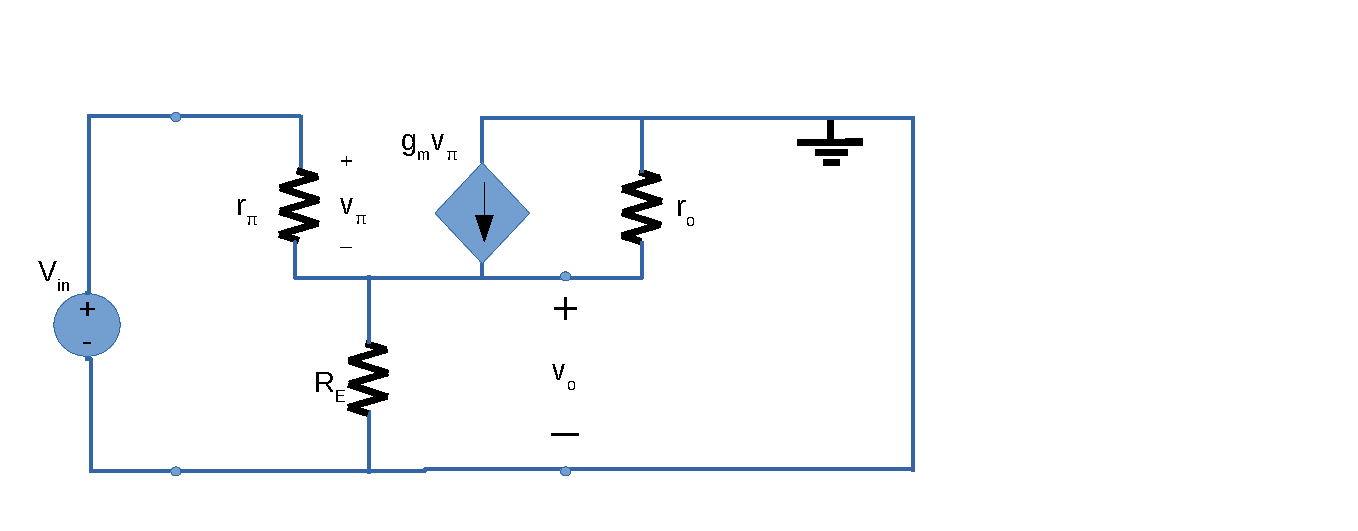
\includegraphics[width=0.8\linewidth]{incrementalos.pdf}
\caption{Output Stage Circuit}                                     %%%%%%%%%%LEGENDA
\label{fig:osincrem}
\end{figure}

Starting by calculating the gain, after analyzing the circuit, we obtain the following equation: 
\begin{equation}
	A_v=\frac{v_o}{v_{in}}=\frac{g_m}{g_\pi+g_E+g_o+g_m}
\end{equation}
, where $g_\pi$, $g_E$ and $g_o$ are the admittances of the respective resistors.

Table~\ref{tab:osav} presents the results and, as predicted, we obtained almost unitary gain.

\begin{table}[H]
  \centering
  \begin{tabular}{|l|r|}
     \hline    
    {\bf Name} & {\bf Value} \\ \hline   
    $A_{V2}$ & 9.736018e-01 dB\\ \hline

  \end{tabular}
  \caption{Gain - Output Stage}
  \label{tab:osav}
\end{table}

In order to obtain the impedances, we used the following equations:
\begin{equation}
	Z_{I2}=\frac{g_\pi+g_E+g_o+g_m}{g_\pi(g_\pi+g_E+g_o)}
\end{equation}
\begin{equation}
	Z_{O2}=\frac{1}{g_\pi+g_E+g_o+g_m}
\end{equation}

The results are presented in Table~\ref{tab:osz}

\begin{table}[H]
  \centering
  \begin{tabular}{|l|r|}
     \hline    
    {\bf Name} & {\bf Value} \\ \hline   
    $Z_{I2}$ & 4.431714e+05 Ohm\\ \hline
$Z_{O2}$ & 5.011041e+01 Ohm\\ \hline

  \end{tabular}
  \caption{Input and Output Impedances - Output Impedances}
  \label{tab:osz}
\end{table}

\subsection{Final}
For the final output, it is important to mention that was used another coupling capacitor between the Output stage and the load.
So, these outputs are in Table~\ref{tab:finaltab}.

\begin{table}[H]
  \centering
  \begin{tabular}{|l|r|}
     \hline    
    {\bf Name} & {\bf Value} \\ \hline   
    $A_{V}$ & 3.647396e+01 dB\\ \hline
$Z_{I}$ & 1.998186e+03 Ohm\\ \hline
$Z_{O}$ & 5.393985e+01 Ohm\\ \hline

  \end{tabular}
  \caption{Output Values}
  \label{tab:finaltab}
\end{table}

This way, the theoretical value of the lower cut-off frequency finally is presented in Table~\ref{tab:lc}.

\begin{table}[H]
  \centering
  \begin{tabular}{|l|r|}
     \hline    
    {\bf Name} & {\bf Value} \\ \hline   
    $Lower CO freq$ & 4.156647e+00 Hz\\ \hline

  \end{tabular}
  \caption{Lower Cut-Off Frequency}
  \label{tab:lc}
\end{table}


